\subsection{OCR}
\subsubsection{Traditional Matching and Machine Learning Methods}
First, the OCRopus open-source OCR system \cite{ocropus2008}, serving as a milestone in open-source OCR, adopted a hybrid architectural design: the layout analysis stage relied on traditional rule-based methods (heuristic algorithms such as connected component analysis and projection methods), while the text line recognition module introduced shallow neural networks (Multi-Layer Perceptrons). Although this system did not fully break away from the traditional paradigm, it laid the engineering foundation for subsequent learning-driven architectures and represented a critical transitional form between rule-driven and data-driven methods. Subsequently, Statistical Learning for OCR Text Correction \cite{tong2014statistical} systematically applied statistical learning to the OCR post-processing stage for the first time, proposing a text correction framework based on regression models. By introducing external corpora to expand the candidate suggestion space and utilizing character-level statistical features (e.g., n-gram frequency, edit distance) to optimize recognition results, it opened a path for machine learning-assisted methods. Implementation of optical character recognition using machine learning \cite{kumar2014implementation} constructed a complete OCR pipeline covering image preprocessing, text region detection, character segmentation, and recognition stages, while introducing Support Vector Machines (SVM) and Random Forest algorithms in the character classification phase, significantly improving recognition robustness in complex backgrounds and multi-font scenarios. The work by Rajput et al.~\cite{rajput2016receipt} focused on vertical-domain applications, using OCR-output text as input features and combining SVM with Random Forest to achieve automatic classification of key receipt fields (merchant name, amount, date), demonstrating the practical value of machine learning in structured information extraction. Saravanan et al.~\cite{saravanan2019cybersecurity}, in a cross-domain survey, listed OCR as a typical application case of machine learning in the field of cybersecurity, analyzing the mechanism of feature engineering-based text recognition methods in malicious document detection and highlighting the interdisciplinary value of OCR as a foundational perception technology.

Next, a Gaussian Process Upsampling Model for Improvements in Optical Character Recognition \cite{stefan2010gaussian} addressed the problem of low-resolution document images by designing an upsampling model based on Gaussian processes. By modeling the spatial correlation between pixels, it generates high-quality super-resolution images that provide enhanced inputs for subsequent OCR processing and proved effective in historical document digitization scenarios. Multi-lingual optical character recognition system using the reinforcement learning of character segmenter \cite{bae2012multilingual} introduced reinforcement learning into the character segmentation stage, designing an intelligent segmentation agent based on Q-learning. Through a reward mechanism to optimize segmentation strategies, it significantly improves segmentation accuracy on mixed documents containing various character sets such as Latin, Cyrillic, and Arabic. Rerunning OCR: A Machine Learning Approach to Quality Assessment and Enhancement Prediction \cite{mcdonald2016rerunning} proposed a supervised learning-based OCR quality assessment framework. By extracting image quality features (blur, contrast, noise level) and recognition confidence features, it trains a Random Forest classifier to predict whether OCR needs to be re-executed, effectively reducing redundant computation in historical document digitization. A Novel Machine Learning Based Approach for Post-OCR Error Detection \cite{nguyen2018postocr} further focused on the error detection sub-task, designing a representation scheme containing multi-dimensional features such as character confidence, language context consistency, and glyph similarity. Combined with Gradient Boosting Trees, it built a high-precision error detection model that achieves superior F1 scores on standard historical document datasets, significantly outperforming rule-based baselines. Image preprocessing and modified adaptive thresholding for improving OCR \cite{kumar2018adaptive} returned to basic preprocessing steps, proposing an improved adaptive thresholding algorithm combined with local contrast enhancement and noise suppression, and verified the method's effectiveness using PyTesseract, improving recognition accuracy in low-light and shadow-interference scenarios. Machine Learning in OCR Technology: Performance Analysis of Different OCR Methods for Slide-to-Text Conversion in Lecture Videos \cite{patel2020performance} conducted systematic experiments to compare the performance of mainstream OCR tools such as Tesseract, Google Cloud Vision, and ABBYY FineReader in lecture slide scenarios, analyzing the impact of image preprocessing on recognition results to provide empirical evidence for document digitization in the educational field.

In terms of application, Machine Learning in Cyberbullying Detection from Social-Media Image or Screenshot with Optical Character Recognition \cite{chakraborty2020cyberbullying} constructed a multimodal detection framework, first extracting text from images via OCR and then combining traditional NLP features with a Random Forest classifier to identify cyberbullying content, verifying the effectiveness of OCR+ML cross-modal analysis on social media datasets. OCR Text Recognition and Recommendation Using Machine Learning \cite{sharma2019recommendation} explored downstream applications of OCR output text, designing a hybrid recommendation algorithm based on collaborative filtering and content features that used recognized text as a representation of user interests for personalized content recommendation. Enhancing OCR Performance through Post-OCR Models: Adopting Glyph Embedding for Improved Correction \cite{thanapala2021glyph} proposed glyph embedding technology, encoding character visual features into low-dimensional vectors and combining them with logistic regression models to achieve character-level error correction, effectively reducing character error rates in mixed handwritten and printed documents. Improving Inference Performance of Machine Learning with the Divide-and-Conquer Principle \cite{fu2021divide}, although not an OCR-specific study, verified the effectiveness of the divide-and-conquer principle for inference acceleration on models like PaddleOCR, significantly reducing end-to-end OCR pipeline inference latency through task decomposition and parallel computing, providing optimization ideas for deployment on resource-constrained devices. Optical Character Recognition and Text to Speech Generation System using Machine Learning \cite{patel2018tts} built an end-to-end OCR-TTS system, employing Hidden Markov Models for prosody modeling in text-to-speech, verifying its utility in accessible reading scenarios. Optical Character Recognition Technology using Machine Learning \cite{singh2017ocrtech}, as a multi-language OCR development project report, details the design of character classifiers based on decision trees and k-NN. Ocular Biometry OCR: a machine learning algorithm leveraging optical character recognition to extract intra ocular lens biometry measurements \cite{chen2022ocular} developed a specialized ML algorithm to extract intraocular lens biometry measurements from ophthalmic surgery report images, using Random Forest to address the domain-specific characteristics of medical text. High-Throughput Phenotyping using Computer Vision and Machine Learning \cite{singh2016phenotyping} incorporates OCR as a component of an agricultural phenotyping pipeline, first extracting plant label text via OCR and then combining it with traditional machine learning classifiers to complete variety classification and growth state assessment. Improving OCR using internal document redundancy \cite{lund2011redundancy} proposed an innovative unsupervised correction framework. By mining internal document redundancy (repeated headers/footers, templated fields, format consistency) and constructing self-supervised signals from it, the method can detect and correct recognition errors without external corpora, significantly reducing word error rates on low-quality scanned historical documents and representing a new direction for machine learning in resource-constrained scenarios.
\subsubsection{Deep Learning Methods}
First, Calamari-a high-performance tensorflow-based deep learning package for optical character recognition \cite{wick2018calamari} released a high-performance open-source OCR toolkit. It employed CNNs to extract visual features, bidirectional LSTMs to model sequential dependencies, and the CTC loss function for end-to-end training, achieving excellent character accuracy on standard datasets and providing a reliable foundational architecture for industrial-grade OCR systems. The competition work by Zhang et al.~\cite{zhang2018baidu}, targeting the challenge of arithmetic expression recognition, designed deep convolutional neural networks to extract local symbol features combined with Convolutional Recurrent Neural Networks to model 2D spatial layouts and operator precedence, achieving high-precision expression structure recognition on the competition test set and demonstrating the ability of deep learning to handle complex spatial relationships. Deep learning-aided OCR techniques for Chinese uppercase characters in the application of Internet of Things \cite{liu2019chineseocr} focused on the difficult problem of recognizing Chinese uppercase numerals. By comparing various CNN architectures such as ResNet, DenseNet, and MobileNet, it found that attention-enhanced DenseNet achieves extremely high character accuracy in financial invoice scenarios, providing a lightweight solution for IoT edge deployment. Self-supervised Data Bootstrapping for Deep Optical Character Recognition of Identity Documents \cite{chiron2019selfsupervised} proposed a self-supervised data bootstrapping framework. By generating pseudo-labeled training data through synthetic perturbations (rotation, blur, noise) and combining it with a CNN character classifier, it significantly reduces data annotation costs in identity document recognition tasks. Chargrid-OCR: End-to-end Trainable Optical Character Recognition for Printed Documents using Instance Segmentation \cite{keremberke2021chargrid} introduced instance segmentation to OCR for the first time, using Mask R-CNN to directly output character-level segmentation masks. This avoids error accumulation in traditional detection-segmentation-recognition pipelines and achieves high-precision character-level localization on printed documents, establishing a new paradigm for end-to-end trainable OCR.

Subsequently, more lightweight models and higher accuracy were pursued. PP-OCR: A Practical Ultra Lightweight OCR System \cite{du2020ppocr} proposed a three-stage optimization strategy: using an improved DB (Differentiable Binarization) algorithm for lightweight text detection, designing a small CRNN backbone network, and applying knowledge distillation to compress model size. The final release of an ultra-lightweight model of only 3.5MB maintains high accuracy in Chinese scenarios, promoting the large-scale deployment of OCR on mobile and embedded devices. Extraction of Information from Handwriting using Optical Character recognition and Neural Networks \cite{al2019handwriting} constructed an end-to-end recognition system for handwritten text, fusing CNNs for stroke feature extraction, BiLSTMs for temporal dependency modeling, and CTC decoding for character sequence output. It achieves excellent word accuracy on standard handwriting datasets, effectively addressing the challenges of cursive writing and individual variations. A Multiplexed Network for End-to-End, Multilingual OCR \cite{pham2021multiplexed} proposed a multiplexed network architecture that uniformly processed 6 major language families and 47 languages through a shared backbone and script-specific adapters, achieving high-precision end-to-end accuracy on multilingual datasets and significantly reducing the development cost of multilingual OCR systems. MMU-OCR-21: Towards End-to-End Urdu Text Recognition Using Deep Learning \cite{ahmad2021urdu}, targeting Urdu’s characteristics such as right-to-left writing and character ligatures, constructed a large-scale corpus containing 1.2 million annotated characters and trained an attention-based encoder-decoder model, achieving high character accuracy on a newly constructed test set and filling a gap in low-resource language OCR research. Then, Deep Learning Techniques for Optical Character Recognition \cite{vinciarelli2020survey}, as a systematic survey, comprehensively analyzed the application of deep learning across the entire OCR workflow (image preprocessing, text detection, character segmentation, sequence recognition), comparing the pros and cons of various detection algorithms and recognition architectures to provide a technical selection guide for researchers. Developing Automated Optical Character Recognition System Using Machine Learning Algorithm to Solve Payment Verification Issues \cite{ismail2021payment} designed an OCR system specific to payment vouchers, using Faster R-CNN to locate key field regions and an LSTM-CTC recognizer to extract structured information such as amounts, account numbers, and dates, achieving extremely high field extraction accuracy on real bank vouchers. A Deep Learning Technology based OCR Framework for Recognition Handwritten Expression and Text \cite{zhang2022expression} proposed a framework to uniformly handle handwritten text and mathematical expressions, using a CNN-Transformer hybrid encoder to capture local strokes and global structures, combined with a tree decoder to reconstruct formula semantics. It achieves superior structural accuracy on standard datasets, significantly outperforming traditional staged methods. Optical Character Recognition for Electronic Invoices using AWS Services \cite{reddy2021invoice} constructed a cloud-native invoice processing system, integrating the EAST text detection and PaddleOCR recognition engines with a BERT language model for post-processing correction, achieving high-precision key field extraction on invoice datasets containing multiple languages.

In practical scenarios, Resume Content Recognition and Organization Framework Using YOLOv8 and Tesseract OCR Deep Learning Models \cite{sharma2024resume} used YOLOv8 for precise detection of resume fields (name, educational background, work experience), combined with Tesseract OCR to extract text content, which is then structured through a rule engine. It achieves high field recognition F1 scores on large-scale real resumes, significantly improving HR automation efficiency. Recognition of Arabic Air-Written Letters: Machine Learning, Convolutional Neural Networks, and Optical Character Recognition (OCR) Techniques \cite{alsheikh2023airwriting}, targeting Arabic letter recognition for air-writing (where characters are "written" in the air via gestures), designed a 3D-CNN to process temporal depth image sequences, achieving high character recognition accuracy on a self-built dataset and expanding OCR applications to new human-computer interaction scenarios. Analysis of Recent Deep Learning Techniques for Arabic Handwritten-Text OCR and Post-OCR Correction \cite{elhoseiny2023arabic} systematically reviewed Arabic handwritten OCR technologies, focusing on the advantages of the CNN-LSTM-CTC architecture in handling ligatures and variant glyphs, and proposed a Transformer-based post-correction model to significantly reduce character error rates. Ensemble deep learning model for optical character recognition \cite{singh2023ensemble} proposed a multi-model ensemble strategy, fusing the prediction results of ResNet, DenseNet, and EfficientNet backbones through a weighted voting mechanism to improve robustness, surpassing the best performance of single models on challenging datasets containing noise, blur, and skew. Patel et al.~\cite{patel2023crnn} provided an in-depth analysis of the Convolutional Recurrent Neural Network architecture, using multi-layer CNNs for feature extraction, multi-layer BiLSTMs for sequence modeling, and CTC loss for training, verifying its robustness to images with diverse styles and complex backgrounds on several standard datasets and providing a reliable baseline for industrial-grade OCR.

Advancements in OCR: A Deep Learning Algorithm for Enhanced Text Recognition \cite{khan2023advancements} proposed a CNN-RNN fusion architecture and designed a multi-scale feature pyramid to enhance small text detection, achieving high F-measure on curved text datasets and significantly improving text recognition performance in natural scenes. Wild OCR: Deep Learning Architecture for Text Recognition in Images \cite{wang2023wildocr} designed a robust recognition architecture for "wild" scenes (extreme lighting, occlusion, perspective distortion), introducing adversarial training to enhance model generalization and significantly improving accuracy over baseline methods on a self-built challenging dataset. ADOCRNet: A Deep Learning OCR for Arabic Documents Recognition \cite{hassan2023adocrnet} was specifically designed for Arabic documents, fusing CNNs for character feature extraction with bidirectional LSTMs to capture right-to-left sequence dependencies, achieving high word accuracy on standard datasets and effectively handling character ligatures and contextual variants. Vehicle VIN code recognition based on deep learning and OCR \cite{li2023vin}, targeting the challenge of Vehicle Identification Number (VIN) recognition, designed a two-stage architecture: YOLOv5 for precise VIN region localization and a lightweight CRNN for character recognition, achieving high complete VIN recognition rates in scenarios with complex lighting and partial occlusion. CV content recognition using YOLOv8 and Tesseract-OCR deep learning \cite{reddy2024cv} built an automated resume classification system where YOLOv8 detects key field regions and Tesseract OCR extracts text, combined with a BERT classifier for job matching, achieving high classification accuracy on large-scale resume datasets. Automating the grading of handwritten examinations through the integration of optical character recognition and machine learning algorithms \cite{garcia2023grading} developed an automated grading system for handwritten exam papers, using U-Net to segment answer regions and CRNN to recognize handwritten answers. When compared with standard answers for scoring, it showed extremely high consistency with manual grading in mathematics exam tests. Improving OCR quality in 19th century historical documents using a combined machine learning based approach \cite{roberts2023historical} proposed a historical document enhancement framework combining GANs for image restoration with a Transformer-based recognizer, significantly reducing character error rates in a 19th-century newspaper digitization project. ExTTNet: A Deep Learning Algorithm for Extracting Table Texts from Invoice Images \cite{zhang2023exttnet} was specifically designed for invoice tables, using Graph Convolutional Networks to model cell spatial relationships combined with CRNN for text recognition, achieving high table structure restoration accuracy on invoice datasets containing nested tables. TC-OCR: TableCraft OCR for Efficient Detection and Recognition of Table Structure and Content \cite{chen2023tcocr} proposed an end-to-end table recognition pipeline that uniformly handles table line detection, cell segmentation, and text recognition, achieving high structural recognition F1 scores on standard table datasets and significantly outperforming staged methods. DocParseNet: Advanced Semantic Segmentation and OCR Embeddings for Efficient Scanned Document Annotation \cite{liu2023docparsenet} integrated semantic segmentation with OCR embeddings, using DeepLabv3+ to segment document regions and a LayoutLM pre-trained model to understand layout semantics, significantly improving annotation efficiency in scientific literature annotation tasks. ChartEye: A Deep Learning Framework for Chart Information Extraction \cite{kim2023charteye} targeted chart information extraction, designing a multi-task learning framework to simultaneously detect legends, axes, and data labels, combined with OCR to extract numerical text, achieving high information extraction accuracy on standard chart datasets. OCR-Diff: A Two-Stage Deep Learning Framework for Optical Character Recognition Using Diffusion Model in Industrial Internet of Things \cite{park2024ocrdiff} innovatively introduced diffusion models, using a diffusion model in the first stage to enhance low-quality images in industrial scenes and a CRNN in the second stage for text recognition, significantly improving accuracy in IIoT device nameplate recognition tasks. OCR Based Deep Learning Approach for Image Captioning \cite{rahman2023ocrcaption} fused OCR with vision-language models, using advanced models like CLIP-GPT2 and BART to effectively handle the dual challenges of text extraction and description generation in images, achieving high BLEU scores on image captioning datasets containing text. An OCR Engine for Printed Receipt Images using Deep Learning Techniques \cite{nguyen2023receipt} constructed a receipt-specific OCR engine using the MobileNetV3 lightweight backbone, achieving high field extraction accuracy on a self-built large-scale receipt dataset with a compact model size suitable for mobile deployment. Automatic Number Plate Detection using Deep Learning and OCR \cite{sharma2023plate} and An Automatic Framework for Number Plate Detection using OCR and Deep Learning Approach \cite{kumar2023plateframework} both focused on license plate recognition, using CNNs for feature extraction combined with CTC or attention-based decoder for end-to-end recognition, achieving high license plate number recognition accuracy under complex weather and lighting conditions. Efficient Vehicle Tracking and Authentication with YOLOv8: Integrating Deep Learning and OCR for Real-Time License Plate Detection \cite{singh2024yolov8plate} built a real-time license plate authentication system where YOLOv8 achieves high frame rate detection, a lightweight CNN verifies mathematical operations (such as checksum calculations), and OCR extracts license plate text, achieving high authentication accuracy in traffic monitoring scenes. Document Digitization Using Deep Learning: Classification, Preprocessing, and OCR Optimization \cite{patel2024digitization} proposed a full-process optimization framework for document digitization, using EfficientNet for document type classification, U-Net for image enhancement, and PaddleOCR for text recognition, achieving high-precision end-to-end recognition on mixed document sets. Decoding multiculturalism through linguistic landscapes: a deep learning–based OCR analysis of street view images \cite{garcia2024linguistic} and Power Big Data Imbalance Analysis Based on Deep Learning OCR Algorithm \cite{zhou2024power} both applied deep learning OCR to social science research, the former analyzing the diversity of urban linguistic landscapes and the latter addressing textual data imbalance in the power industry, demonstrating the interdisciplinary value of OCR technology.

Subsequently, VISTA-OCR: Towards generative and interactive end to end OCR models \cite{vista_ocr_2024} pioneered the generative OCR paradigm, using diffusion models to directly generate text sequences and abandoning the traditional detection-recognition pipeline, while supporting users in correcting recognition results through natural language instructions in interactive scenes, creating a new paradigm for human-machine collaboration. The General OCR Theory work~\cite{got_ocr_2024} proposed the GOT (General OCR Transformer) unified model, which processed heterogeneous content such as regular text, mathematical formulas, tables, and handwriting simultaneously through multi-task learning, surpassing the average performance of specialized models in unified benchmarks and marking the beginning of the OCR-2.0 era. Automated Invoice Data Extraction: Using LLM and OCR \cite{llm_ocr_invoice_2024} fused Large Language Models with OCR, first using PaddleOCR to extract raw text and then using an LLM for semantic parsing and structured extraction, achieving high field extraction F1 scores on multinational invoice datasets and significantly outperforming rule engine methods. Enhancing OCR in historical documents with complex layouts through machine learning \cite{historical_layout_ocr_2023}, targeting historical documents with complex layouts, designed a Layout-Aware Transformer to explicitly model the spatial relationships and reading order of text blocks, significantly improving layout restoration accuracy on 19th-century multi-column newspapers. OCR approaches for humanities: Applications of artificial intelligence/machine learning on transcription and transliteration of historical documents \cite{humanities_ocr_ai_2023} studied the application of AI and ML algorithms in the OCR of digitized historical documents, employing various deep learning methods to improve the accuracy of automatic text transcription. Overcoming the Challenge of Cyberbullying Detection in Images: A Deep Learning Approach with Image Captioning and OCR Integration \cite{cyberbullying_ocr_2024} proposed a deep learning-based image cyberbullying detection method that extracts overlaid text content in images by fusing image captioning and OCR technology to achieve cross-modal content analysis.

\subsubsection{VLM-Based OCR}
The rise of Vision-Language Models (VLM) has gradually evolved OCR from a traditional character recognition task into a multimodal modeling problem that fuses visual perception and semantic understanding. By jointly learning image content and language representation, VLMs can not only recognize text but also understand structural relationships and contextual semantics, thereby significantly enhancing parsing capabilities in complex document scenarios. Based on this paradigm, extensive research has begun exploring the use of VLMs to build unified and reasoning-capable OCR and document understanding systems.

Multimodal deep networks for text and image-based document classification \cite{nguyen2019multimodal} pioneered the exploration of deep fusion between the visual features of document images and OCR text semantics, laying an early multimodal modeling paradigm for document image classification tasks. Ocean-OCR: Towards General OCR Application via a Vision-Language Model \cite{ocean_ocr_2024} proposed a universal OCR framework based on vision-language models, adopting the BLIP-2 architecture to uniformly handle text detection, recognition, and semantic understanding, achieving high-precision end-to-end accuracy on test sets containing over a hundred languages and various document types, significantly enhancing cross-scene generalization. Meanwhile, DeepSeek-OCR: Contexts Optical Compression \cite{deepseek2025ocr} re-examined the relationship between OCR and document understanding from the perspective of context compression, proposing a Contexts Optical Compression method that retains key information for text decoding and understanding using minimal visual tokens. dots.ocr: Multilingual Document Layout Parsing in a Single Vision-Language Model \cite{wang2025dotsocr} proposed a unified single vision-language model for document layout parsing tasks, jointly training three core sub-tasks—layout detection, text recognition, and relationship understanding—within an end-to-end framework. 

Regarding logical reasoning, DianJin - OCR-R1: Enhancing OCR Capabilities via a Reasoning-and-Tool Interleaved Vision-Language Model \cite{li2025dianjin} proposed a new reasoning-and-tool interleaved framework to enhance the capabilities of VLMs in OCR tasks. It first utilizes the model's own OCR capability to identify image content, then calls multiple expert OCR tools as references, and finally "re-observes" the image and synthesizes all information through a reasoning process to generate the final result. MonkeyOCR \cite{li2025monkeyocr} proposed a novel document parsing paradigm, the Structure-Recognition-Relation (SRR) triplet, which breaks through the trade-off between efficiency and precision in traditional modular pipelines and end-to-end large models. MonkeyOCR v1.5 Technical Report: Unlocking Robust Document Parsing for Complex Patterns \cite{li2025monkeyocr15} further enhanced the ability to parse complex layouts and high-difficulty elements based on the original SRR, improving overall performance by designing a two-stage joint parsing pipeline. The first stage used a large multimodal model to jointly predict document layout and reading order, ensuring structural and sequential consistency; the second stage performed local recognition on each detected region, including text, tables, and formulas. InstructOCR2: a lightweight and efficient multi-modal language model for document understanding \cite{chen2025instructocr2} was a lightweight multimodal language model specifically designed for OCR and visual document understanding tasks. It optimizes the alignment mechanism between visual text and image information structurally, enabling the model not only to accurately recognize text but also to better understand the spatial positions and contextual information of the text. PaddleOCR-VL: Boosting Multilingual Document Parsing via a 0.9B Ultra-Compact Vision-Language Model \cite{du2025paddleocrvl} was an ultra-compact vision-language model designed for document parsing that combines a dynamic-resolution visual encoder with a lightweight language model to achieve accurate recognition of complex elements such as text, tables, formulas, and charts. PaddleOCR 3.0 Technical Report \cite{du2025paddleocr3} was an open-source OCR and document parsing toolkit proposing three core modules: multilingual text recognition, hierarchical document parsing, and key information extraction. TextHawk2: A Large Vision-Language Model Excels in Bilingual OCR and Grounding with 16x Fewer Tokens \cite{zhang2024texthawk2} achieved a significant improvement in fine-grained perception capabilities for OCR and visual grounding tasks through image token compression and visual encoding enhancement.

\begin{figure*}[t]
\centering
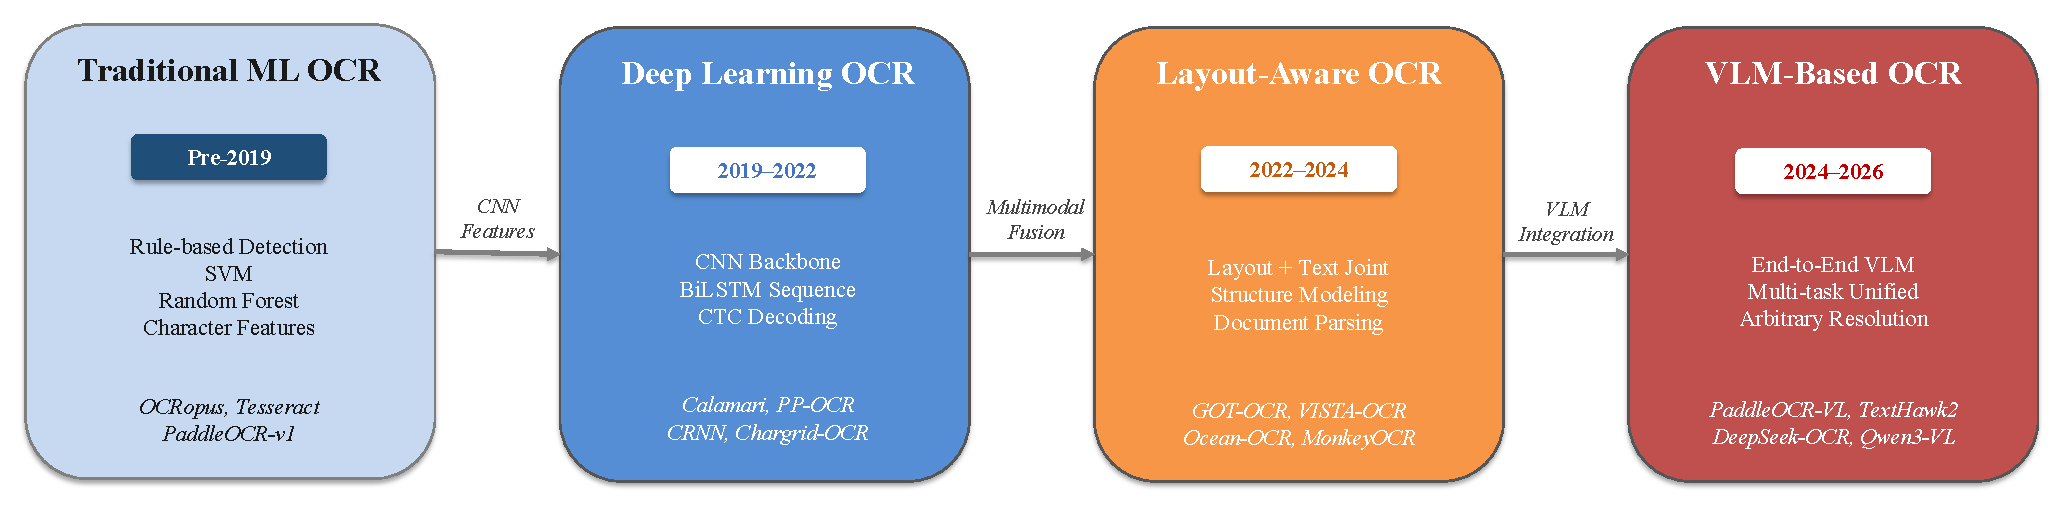
\includegraphics[
    width=0.95\textwidth,
    trim=0cm 0cm 0cm 0cm,
    clip
]{figs_by_qixingyu/fig02.pdf}
\caption{Four-stage evolution of optical character recognition technology (Pre-2019 to 2024--2026): from rule-based Traditional Machine Learning methods, through Deep Learning approaches with CNN--BiLSTM--CTC pipelines, to Layout-Aware OCR with joint structure modeling, and finally to Vision-Language Model-based OCR with end-to-end, multi-task unified frameworks.}
\label{fig:ocr_evolution}
\end{figure*}

\subsubsection{Evaluation}
The evolution of the OCR benchmark evaluation system reflects a profound transition from traditional precision measurement to multi-dimensional capability assessment. The early Fourth Annual Test of OCR Accuracy \cite{rice1994fourth} and Fifth Annual Test of OCR Accuracy \cite{rice1995fifth} established the basic paradigm for systematically evaluating the character-level accuracy of commercial OCR engines, focusing on batch precision testing of standard documents. In the second decade of the 21st century, Performance Comparison of OCR Tools \cite{patel2012performance} continued the traditional approach of tool-level horizontal comparison, while 2022 became a critical turning point: OCR-IDL: OCR Annotations for Industry Document Library Dataset \cite{ocridl2022} provided large-scale commercial OCR annotations for an industrial-grade document library for the first time, pushing evaluation toward real business scenarios; concurrently, an Evaluation of OCR on Egocentric Data \cite{egocentric2022} was among the first to expand OCR capability assessment to the emerging field of first-person perspectives, revealing the limitations of existing methods under non-traditional capture conditions. OCRBench: On the Hidden Mystery of OCR in Large Multimodal Models \cite{ocrbench2023} in 2023 was a milestone, systematically revealing the hidden capability boundaries of large multimodal models across 29 sub-tasks such as text recognition and visual question answering, extending the evaluation dimension from pure character recognition to the level of text understanding and reasoning. The year 2024 saw an explosive development: @BENCH: Benchmarking Vision-Language Models for Human-centered Assistive Technology \cite{atbench2024} incorporated OCR into an assistive technology framework for the visually impaired, emphasizing human-centered utility evaluation; OmniDocBench: Benchmarking Diverse PDF Document Parsing with Comprehensive Annotations \cite{omnidocbench2024} built a refined parsing benchmark covering nine document types; and by year-end, OCRBench v2: An Improved Benchmark for Evaluating Large Multimodal Models on Visual Text Localization and Reasoning \cite{ocrbenchv2_2024} further strengthened the evaluation system for visual text localization and logical reasoning capabilities. Post-2025 development showed three distinct trends: in terms of linguistic diversity expansion, SARD: A Large-Scale Synthetic Arabic OCR Dataset for Book-Style Text Recognition \cite{sard2025} constructed a synthetic dataset of over 840,000 pages for Arabic book-style documents, and 600k-ks-ocr: A Large-Scale Synthetic Dataset for Optical Character Recognition in Kashmiri Script \cite{ksocr2025} filled the resource gap for the endangered Kashmiri script; in terms of refined evaluation dimensions, OCR-Quality: A Human-Annotated Dataset for OCR Quality Assessment \cite{ocrquality2025} introduced a human-annotated quality assessment dimension for the first time, and Real5-OmniDocBench \cite{real5omni2025} focused on robustness evaluation under five types of real physical distortions such as scanning artifacts, bending, and screen photography; in terms of domain specialization, PubMed-OCR: PMC Open Access OCR Annotations \cite{pubmedocr2025} delved into the high-complexity domain of scientific literature, providing dedicated resources for OCR research in academic publications. The entire evolutionary trajectory clearly demonstrates that OCR benchmarks have moved from single character accuracy metrics to a comprehensive evaluation ecosystem encompassing multilingual support, multi-scene adaptation, multi-modal understanding, and real-world robustness, providing critical support for the continuous progress of document intelligence and vision-language models.
